% Superday Topic B -- final deck (2026-11-01): C08 as the final design; C01-C07 as the hypotheses it replaced.  XeLaTeX x2.
% Facts: research/coldstart_C01..C08 PLAN.md and RESULT.md, research/coldstart_C08/final.json.  Layout: talk/superday/OUTLINE.md.
\documentclass[t,20pt]{beamer}
\geometry{paperwidth=13.333in,paperheight=7.5in}

% Metropolis inner / outer / colour themes; fonts are set below (Fira Sans + Fira Math from the TeX tree).
\useinnertheme[sectionpage=none,subsectionpage=none]{metropolis}
\useoutertheme[progressbar=none,numbering=none]{metropolis}
\usecolortheme{metropolis}
\usefonttheme{professionalfonts}

\usepackage{fontspec}
\usepackage{unicode-math}
\setsansfont{FiraSans}[Extension=.otf, UprightFont=*-Book, ItalicFont=*-BookItalic,
  BoldFont=*-SemiBold, BoldItalicFont=*-SemiBoldItalic]
\setmainfont{FiraSans}[Extension=.otf, UprightFont=*-Book, ItalicFont=*-BookItalic,
  BoldFont=*-SemiBold, BoldItalicFont=*-SemiBoldItalic]
\setmonofont{FiraMono}[Extension=.otf, UprightFont=*-Regular, BoldFont=*-Medium]
\newfontfamily\mediumfont{FiraSans}[Extension=.otf, UprightFont=*-Medium, ItalicFont=*-MediumItalic]
\setmathfont{FiraMath-Regular.otf}
\newfontfamily\cjkfont{FandolHei-Regular.otf}   % only for one Chinese file name in a source note

\usepackage{tikz}
\usetikzlibrary{arrows.meta,positioning,calc,fit,decorations.markings}
\usepackage{array,booktabs,colortbl}
\usepackage{fancyvrb}

% ------------------------------------------------------------------ colours (OUTLINE.md)
\definecolor{ink}{HTML}{2E2E2E}
\definecolor{sec}{HTML}{6B6B6B}
\definecolor{rulec}{HTML}{C8C8C8}
\definecolor{accent}{HTML}{1F5A96}
\setbeamercolor{normal text}{fg=ink,bg=white}
\setbeamercolor{background canvas}{bg=white}
\setbeamercolor{frametitle}{fg=ink,bg=white}
\setbeamercolor{alerted text}{fg=accent}
\setbeamercolor{structure}{fg=ink}
\arrayrulecolor{rulec}
\setlength{\heavyrulewidth}{0.9pt}
\setlength{\lightrulewidth}{0.9pt}

% ------------------------------------------------------------------ sizes (points are literal: the page is 13.333 x 7.5 in)
\newcommand\titlesize{\fontsize{32}{38}\selectfont}
\newcommand\secsize{\fontsize{16}{20}\selectfont}
\newcommand\nodesize{\fontsize{16}{19}\selectfont\hyphenpenalty=10000\exhyphenpenalty=10000}
\newcommand\notesize{\fontsize{14}{17}\selectfont\hyphenpenalty=10000\exhyphenpenalty=10000}
\newcommand\pnsize{\fontsize{12}{14}\selectfont}
\newcommand\expr[1]{{\ttfamily\fontsize{14}{17}\selectfont\detokenize{#1}}}   % expression in mono, 14 pt, inside tables

% ------------------------------------------------------------------ grid
\setbeamersize{text margin left=0.85in,text margin right=0.85in}
\setbeamertemplate{navigation symbols}{}
\setbeamertemplate{headline}{}
% Frame title: a fixed-height box, baseline 0.92 in from the top on every page (strut fixes the baseline).
\setbeamertemplate{frametitle}{%
  \nointerlineskip
  \vbox to 1.30in{%
    \vskip 0.50in
    \hbox{{\mediumfont\titlesize\color{ink}\rule{0pt}{0.42in}\insertframetitle}}%
    \vss}%
}
% Page number: bottom right, 12 pt, mid-gray, right edge on the right text margin.
\setbeamertemplate{footline}{%
  \hbox to \paperwidth{\hfill{\pnsize\color{sec}\insertframenumber}\hskip 0.85in}%
  \vskip 0.36in}
\setlength{\parindent}{0pt}
\setlength{\parskip}{0pt}

% ------------------------------------------------------------------ text helpers
\newcommand\key[1]{{\mediumfont\color{accent}#1}}
\newcommand\lead[1]{{\mediumfont #1}}
\newcommand\illus{{\notesize\itshape\color{sec}illustrative}}
\newcommand\file[1]{{\ttfamily\detokenize{#1}}}
\newcommand\sub[1]{\par\vspace{5pt}{\raggedright\secsize\color{sec}#1\par}}
\newenvironment{blist}{%
  \begin{list}{\textcolor{sec}{\textbullet}}{\def\makelabel##1{##1\hfil}%
    \setlength\leftmargin{0.34in}\setlength\labelwidth{0.2in}\setlength\labelsep{0.14in}%
    \setlength\itemsep{16pt}\setlength\parsep{0pt}\setlength\topsep{0pt}\setlength\partopsep{0pt}%
    \setlength\itemindent{0pt}\setlength\listparindent{0pt}\setlength\rightmargin{0pt}}}%
  {\end{list}}
\newcounter{nl}
\newenvironment{nlist}{%
  \begin{list}{\textcolor{sec}{\arabic{nl}}}{\usecounter{nl}\def\makelabel##1{##1\hfil}%
    \setlength\leftmargin{0.40in}\setlength\labelwidth{0.26in}\setlength\labelsep{0.14in}%
    \setlength\itemsep{26pt}\setlength\parsep{0pt}\setlength\topsep{0pt}\setlength\partopsep{0pt}%
    \setlength\itemindent{0pt}\setlength\listparindent{0pt}\setlength\rightmargin{0pt}}}%
  {\end{list}}
\newcolumntype{L}[1]{>{\raggedright\arraybackslash}p{#1}}
\newcommand\thead[1]{\leavevmode{\mediumfont\color{sec}#1}}
\newcommand\gap[1]{\par\vspace{#1}}
% content top: tables and figures start on the frame's top line; a first text line or a [t] minipage is lifted onto it
\newcommand\textfirst{\vspace*{-0.14in}}
\newcommand\colsfirst{\vspace*{-0.37in}}
\newcommand\colsafter{\par\vspace{-0.24in}}
% figures sit on the text block: left edge on the left margin, width exactly the text width
\newcommand\fig[1]{\par\noindent\makebox[\textwidth][l]{\input{#1}}\par}
\AtBeginDocument{\hyphenpenalty=10000\exhyphenpenalty=10000\raggedright}

% ------------------------------------------------------------------ figures: one line width, Stealth tips, square corners
\tikzset{
  x=1in, y=1in,
  >={Stealth[length=7pt,width=5.5pt]},
  every picture/.style={line width=0.9pt},
  grid/.style={trim left=0in, trim right=11.633in-0.9pt},
  box/.style={rectangle, draw=ink, line width=0.9pt, minimum height=0.68in, align=center,
              font=\nodesize, text=ink, inner sep=4pt},
  cb/.style={box},                                  % code part
  lb/.style={box, draw=accent},                     % LLM / Partura part
  pb/.style={box, draw=sec, dashed, text=sec},      % planned, not built
  tint/.style={fill=accent!10},                     % the single 10 % accent tint per figure
  arr/.style={->, line width=0.9pt, draw=ink},
  arrl/.style={->, line width=0.9pt, draw=accent},
  lab/.style={font=\nodesize, text=sec, inner sep=2pt},
  labl/.style={font=\nodesize, text=accent, inner sep=2pt},
  ann/.style={font=\notesize, text=sec, inner sep=1.5pt},        % 14 pt figure annotations
  annl/.style={font=\notesize, text=accent, inner sep=1.5pt},
  anni/.style={font=\notesize, text=ink, inner sep=1.5pt},
  guide/.style={draw=rulec, dotted, line width=0.9pt},            % dotted alignment guides
  mask/.style={fill=white},                                       % label background over a line
  t10/.style={fill=accent!10}, t20/.style={fill=accent!20}, t28/.style={fill=accent!28}, t35/.style={fill=accent!35},
}

\newcommand\takeaway[1]{\par\vspace{0.10in}{\fontsize{22}{26}\selectfont\mediumfont\color{accent}#1\par}}
\newcommand\body[1]{{\fontsize{18}{22}\selectfont#1}}
\newcommand\src[1]{\par\vfill{\notesize\color{sec}#1\par}\vspace{0.02in}}
\newcommand\bigmetric[1]{{\mediumfont\fontsize{36}{40}\selectfont\color{accent}#1}}

\begin{document}
\newcolumntype{R}[1]{>{\raggedleft\arraybackslash}p{#1}}

% ================================================================== 1 Title
\begin{frame}[plain]
\begin{tikzpicture}[remember picture,overlay]
  \node[anchor=base west, inner sep=0, align=left, text=ink]
    at ($(current page.north west)+(0.85in,-2.45in)$)
    {\mediumfont\titlesize Partura: an LLM research team\\[2pt]\mediumfont\titlesize that steers a symbolic alpha miner};
  \node[anchor=base west, inner sep=0, text=sec]
    at ($(current page.north west)+(0.85in,-3.45in)$)
    {Eight pre-registered designs; the eighth beat plain GP on a development set};
  \draw[rulec] ($(current page.north west)+(0.85in,-3.85in)$) -- ++(11.633in,0);
  \node[anchor=base west, inner sep=0, text=ink]
    at ($(current page.north west)+(0.85in,-4.45in)$) {Xiangyu Wang};
  \node[anchor=base west, inner sep=0, text=sec, font=\secsize]
    at ($(current page.north west)+(0.85in,-4.90in)$) {Topic B \,·\, 2026-11-01};
\end{tikzpicture}
\end{frame}

% ================================================================== 2 The question
\begin{frame}{Finding an alpha is not evidence that the LLM helped}
\textfirst
\body{A good backtest answers “was something found?” The question here is \key{“did the LLM make search better than search alone?”}}
\gap{0.26in}
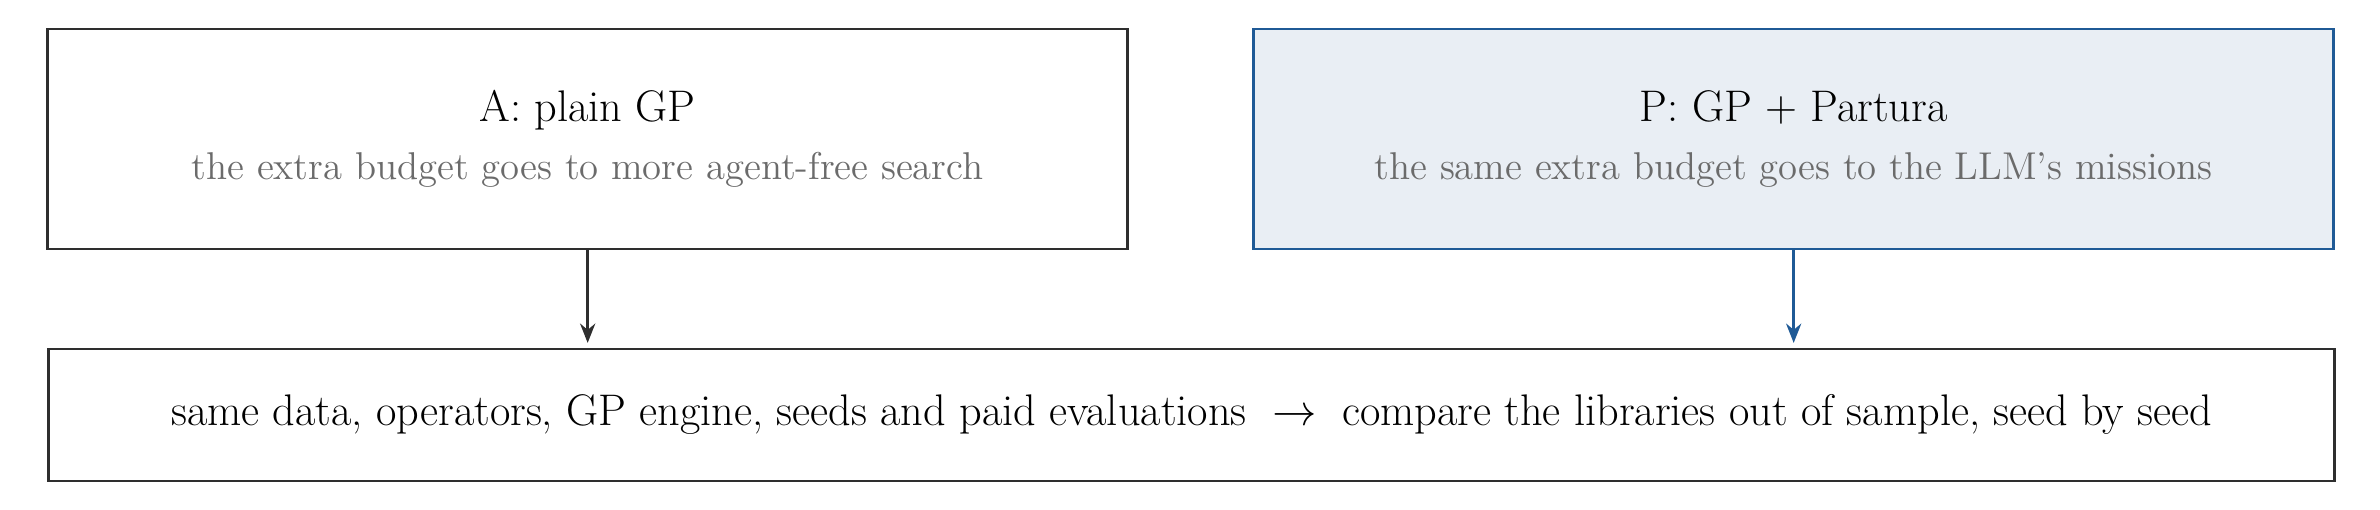
\begin{tikzpicture}[grid]
  \tikzset{px/.style={rectangle, draw=ink, minimum width=5.40in, minimum height=1.10in, align=center, font=\nodesize, inner sep=6pt}}
  \node[px] at (2.80,-0.60) {\mediumfont A: plain GP\\[2pt]{\notesize\color{sec}the extra budget goes to more agent-free search}};
  \node[px, draw=accent, fill=accent!10] at (8.83,-0.60) {\mediumfont P: GP + Partura\\[2pt]{\notesize\color{sec}the same extra budget goes to the LLM's missions}};
  \draw[arr] (2.80,-1.15) -- (2.80,-1.62);
  \draw[arrl] (8.83,-1.15) -- (8.83,-1.62);
  \node[draw=ink, minimum width=11.43in, minimum height=0.66in, align=center, font=\nodesize] at (5.82,-1.98)
    {same data, operators, GP engine, seeds and paid evaluations \;$\rightarrow$\; compare the libraries out of sample, seed by seed};
\end{tikzpicture}
\gap{0.20in}
\takeaway{The baseline is a capable searcher, not “no research”.}
\src{Both arms share the main search M (untouched by any agent). C08: 4,438 paid evaluations for A, 4,525 for P; 8 paired seeds.}
\end{frame}

% ================================================================== 3 Search is cheap
\begin{frame}{Search is cheap; belief is expensive}
\textfirst
\fig{figs_final/cost.tex}
\gap{0.10in}
\takeaway{Tokens should buy beliefs that move thousands of cheap evaluations, not candidates.}
\src{An LLM writing formulas one by one competes with GP at GP's game. Shapes are illustrative, not measured.}
\end{frame}

% ================================================================== 4 Two layers, two directions
\begin{frame}{Two layers, two directions, one referee in code}
\textfirst
\body{The agent proposes where to look; the searcher reports what it found and what failed. \lead{Neither side grades itself.}}
\gap{0.20in}
\fig{figs_final/loop8.tex}
\gap{0.12in}
\takeaway{Reasoning guides search. Search revises reasoning. Code measures both.}
\end{frame}

% ================================================================== 5 Task
\begin{frame}{The task: one formula, one daily signal}
\fig{figs_final/task.tex}
\gap{0.06in}
\body{\lead{Signal} $s_{i,t}=x(\mathcal{D}_{\le t})_i$;\quad \lead{target} $r_{i,t+1}=P_{i,t+2}/P_{i,t+1}-1$, $P$ = first-15-minute VWAP.}
\src{About 5,200 A-share stocks, 8 minute fields, 241 bars a day, 6 daily fields. Search sees 2018-01-02 to 2023-08-07 only. Book: top-decile residual long-only, 15 bp per side.}
\end{frame}

% ================================================================== 6 Final design
\begin{frame}{The final design: the main search runs untouched}
\fig{figs_final/arch8.tex}
\src{Partura cannot ban, reweight or edit M. Each round: two GP slots of 96 evaluations, up to 16 R variants. Schematic.}
\end{frame}

% ================================================================== 7 Agents at bottlenecks
\begin{frame}{An LLM only where judgement is the bottleneck}
\textfirst
\body{Everything that can be measured is measured in code. The LLM is used where a choice has to be made from evidence.}
\gap{0.16in}
\begingroup\secsize
\renewcommand\arraystretch{1.40}%
\begin{tabular}{@{}L{2.45in}L{4.20in}L{4.55in}@{}}
\toprule
\thead{Decision} & \thead{LLM role} & \thead{Referee in code} \\
\midrule
\lead{Where is the alpha?} & round 1: anatomist reads the locate output & heads table, subtree commonality, ablation \\
\lead{What to search next} & PI writes E, R, N missions with seeds & admissibility check; library ban $|\rho| \ge 0.7$ \\
\lead{Is the plan broken?} & auditor: maths errors and duplicates only & correlation table; auto-strike rules \\
\lead{Did it work?} & none & fixed yardstick, paired seeds, ledgered read \\
\bottomrule
\end{tabular}
\endgroup
\gap{0.18in}
\takeaway{Roles are hypotheses about division of labour; C08 dropped two of them.}
\src{C08 rounds 2–3 ran without the anatomist and librarian, with Sonnet as PI and auditor (PLAN revision 1). Models: PI and auditor Opus 5.5 in round 1; checker Haiku 5.5.}
\end{frame}

% ================================================================== 8 One round end to end
\begin{frame}{One round, end to end: seed 808, round 3}
\textfirst
\fig{figs_final/flow8.tex}
\gap{0.16in}
\begingroup\secsize
\renewcommand\arraystretch{1.12}%
\begin{tabular}{@{}L{1.20in}L{10.10in}@{}}
\toprule
\lead{Input} & subtree \expr{ts_mean(day_centroid(Volume), 20)} alone scores +1.28; it is a necessary part of a +0.83 head \\
\lead{Decision} & E slot keeps it as the core (drift, instability, bucketing around it); N slot: shape of the minute-volume distribution \\
\lead{Audit} & E novelty 3, soundness 4, 11 of 12 seeds kept; N 4 / 4, 10 of 12 kept (one seed is liquidity: $|\rho|$ 0.80) \\
\lead{Output} & E found 3 heads; test Sharpe +0.50, +0.39, $-$0.43. N found none \\
\bottomrule
\end{tabular}
\endgroup
\src{Files: loc.md $\to$ missions.yaml $\to$ corr\_1.md, audit\_1.yaml $\to$ evidence.json. Chosen as the last round run, not by result. “Day centroid” = where in the day a stock's volume trades, 0 = open, 1 = close. Sources: research/coldstart\_C08/partura/s808/r3/ (loc.md, missions\_final.yaml, audit\_record.json); final.json.}
\end{frame}

% ================================================================== 9 Verdict rule
\begin{frame}{The verdict rule was fixed before any run}
\textfirst
\begin{blist}\setlength\itemsep{14pt}
  \item \lead{Yardstick:} rank each day first, then smooth; residual on 5 controls and their squares and cubes; top-decile long-only, 15 bp.
  \item \lead{Library per arm:} M's heads plus the arm's own heads, de-duplicated; equal-weight fusion, neutralised once more.
  \item \lead{Primary:} P against A, fused-book test Sharpe, 8 paired seeds, one-sided Wilcoxon, $\alpha = 0.05$: \emph{better, worse, or cannot tell}.
  \item \lead{Test segment} 2023-08-08 to 2025-12-31, read once. \lead{Forward} 2026-01-01 to 2026-09-16: report only.
\end{blist}
\gap{0.16in}
\takeaway{The test segment had been read seven times before: C08's verdict is a development result.}
\src{research/coldstart\_C08/PLAN.md §2–§4, committed before any C08 run; revisions 1–2 changed cost and who ran round 3, not a comparison rule.}
\end{frame}

% ================================================================== 10 Result
\begin{frame}{C08: Partura beat plain GP in 7 of 8 seeds}
\textfirst
\noindent\begin{minipage}[t]{3.60in}\vspace{0pt}
{\secsize\color{sec}median P $-$ A, test segment}\par
\bigmetric{+0.23}\par\vspace{0.02in}
\body{one-sided $p$ = 0.012: \key{P is better}}
\end{minipage}\hfill
\begin{minipage}[t]{3.60in}\vspace{0pt}
{\secsize\color{sec}mean fused book, A / P}\par
\bigmetric{$-$0.33 / +0.16}\par\vspace{0.02in}
\body{evaluations 4,438 / 4,525}
\end{minipage}\hfill
\begin{minipage}[t]{3.60in}\vspace{0pt}
{\secsize\color{sec}forward 2026, report only}\par
\bigmetric{+0.54}\par\vspace{0.02in}
\body{median, 7 of 8 seeds, $p$ = 0.020}
\end{minipage}
\gap{0.16in}
\fig{figs_final/seeds8.tex}
\src{Fused residual-book net Sharpe on the test segment, per seed. 152 of 155 heads reproduce. Source: research/coldstart\_C08/RESULT.md §1–§2; final.json.}
\end{frame}

% ================================================================== 11 What the win is
\begin{frame}{What the win is, and what it is not}
\textfirst
\begingroup\secsize
\renewcommand\arraystretch{1.30}%
\begin{tabular}{@{}L{4.10in}R{1.30in}R{1.55in}L{4.10in}@{}}
\toprule
\thead{Comparison or group} & \thead{Median} & \thead{W / L} & \thead{Reading} \\
\midrule
P against A (verdict) & +0.23 & 7 / 1 & significant, $p$ 0.012 \\
P against M (no extra search) & +0.24 & 5 / 3 & \textcolor{accent}{not significant}, $p$ 0.098 \\
A against M & 0.00 & 2 / 3 & GP's extra heads hurt 3 books \\
P's 55 extra heads, one by one & +0.07 & 32 / 55 $>0$ & the edge is in the book \\
\expr{day_centroid(Volume)} family, 17 heads & +0.03 & 9 / 17 $>0$ & densest in sample; did not hold \\
\bottomrule
\end{tabular}
\endgroup
\gap{0.20in}
\takeaway{Less bad, not more profitable: P's median book is +0.05; A lost $-$1.05 and $-$0.97 on two seeds.}
\src{Readings are inferences after the read, not tests. Round-3 heads did best (10 of 12 positive), round 1 worst (5 of 15), but round and flow are confounded. Source: RESULT.md §3–§4.}
\end{frame}

% ================================================================== 12 Evolution
\begin{frame}{Eight designs, eight hypotheses}
\textfirst
\fig{figs_final/evo.tex}
\gap{0.12in}
\takeaway{Each failure was a hypothesis about where the LLM adds value, and each was rejected on held-out data.}
\src{Every design was pre-registered and judged against plain GP on the same seeds. The sequence is not a performance series: designs changed after reading earlier results. Sources: RESULT.md §1 of each study.}
\end{frame}

% ================================================================== 13 C01-C04
\begin{frame}{Rejected: “the LLM should steer the searcher” (C01–C04)}
\textfirst
\begingroup\secsize
\renewcommand\arraystretch{1.30}%
\begin{tabular}{@{}L{0.85in}L{4.75in}L{5.60in}@{}}
\toprule
\thead{Study} & \thead{How the LLM steered} & \thead{What happened (test segment)} \\
\midrule
\lead{C01} & priors and neighbourhoods reweight GP's proposals & \textcolor{accent}{worse}: valid heads A 19, Partura 13 \\
\lead{C02} & LLM tests its hypotheses, designs the first population & \textcolor{accent}{worse}: new valid heads A 7, Partura 2 \\
\lead{C03} & same, reward only what survives style controls & cannot tell: 0 and 0; no LLM mechanism test passed \\
\lead{C04} & more data; the LLM bans families & cannot tell: its ban killed A's family that held on test \\
\bottomrule
\end{tabular}
\endgroup
\gap{0.20in}
\body{Two lessons: most “valid” heads were style exposure (C01: 19 $\to$ 2 after neutralisation), and \lead{inside a fixed budget, every LLM mistake crowds out exploration.}}
\takeaway{Carried into C08: the main search M is never touched by an agent.}
\src{C04: discoveries 53 (Partura) against 173 (A); median B $-$ A $-$0.17, $p$(worse) 0.11. Sources: research/coldstart\_C01..C04/RESULT.md; talk/superday/DOSSIER.md §3.}
\end{frame}

% ================================================================== 14 C05
\begin{frame}{Rejected: “a better selection score means better alpha” (C05)}
\textfirst
\fig{figs_final/selection.tex}
\gap{0.30in}
\body{Partura added E, R, N missions beside an untouched M. It won selection in 7 of 8 seeds and tied on test (median +0.08, $p$ 0.42).}
\gap{0.08in}
\body{Its extra heads were the weakest one by one: test Sharpe 0.32, against 0.80 for A's.}
\takeaway{Carried into C08: never trust in-sample gains; the floor held because M was untouched.}
\src{Post-read inference: the LLM optimised a leaky reward better (convex transforms rebuilt volatility). Fused residual-book Sharpe, mean of 8 seeds. Source: research/coldstart\_C05/RESULT.md §1–§4.}
\end{frame}

% ================================================================== 15 C06
\begin{frame}{Rejected: “a strict auditor picks better ideas” (C06)}
\textfirst
\body{The auditor caught a real error: the PI read minute VWAP as the bar's close, $\mathrm{day\_cov}\cdot M/\bar P \approx (\theta-\tfrac12)Q - R\delta$, not $Q/2 - R\delta$.}
\gap{0.12in}
\body{As a filter it was wrong-way round:}
\gap{0.10in}
\begingroup\secsize
\renewcommand\arraystretch{1.30}%
\begin{tabular}{@{}L{2.90in}R{1.20in}R{2.25in}R{2.10in}R{2.00in}@{}}
\toprule
\thead{Auditor decision} & \thead{Seeds} & \thead{Mean test Sharpe} & \thead{Test positive} & \thead{Forward} \\
\midrule
accepted & 469 & $-$0.91 & 15\% & $-$0.83 \\
rejected & 162 & \textcolor{accent}{$-$0.53} & \textcolor{accent}{34\%} & $-$0.73 \\
\bottomrule
\end{tabular}
\endgroup
\gap{0.10in}
\body{Accepted beat rejected in only 3 of 24 seed-rounds ($p$ 0.999). Book: cannot tell (median +0.01).}
\takeaway{Carried into C08: the auditor blocks only maths errors and duplicates.}
\src{Seeds are GP starting points read singly, not finished signals. $\theta$ = VWAP's position inside the bar. Source: research/coldstart\_C06/RESULT.md §1, §4.}
\end{frame}

% ================================================================== 16 C07
\begin{frame}{Rejected: “the yardstick was fine” (C07)}
\textfirst
\body{Two leaks paid for control exposure: a convex transform rebuilt volatility, and linear neutralisation left U- and S-shaped exposure.}
\gap{0.10in}
\body{\lead{Fix:} rank first, then smooth; residual on controls, their squares and cubes. Then an LLM only filtered GP's heads:}
\gap{0.14in}
\noindent\begin{minipage}[t]{5.50in}\vspace{0pt}
{\secsize\color{sec}fused book, verifier against A}\par\vspace{0.04in}
\bigmetric{+0.11}\par\vspace{0.04in}
\body{median, $p$ 0.062: cannot tell}
\end{minipage}\hfill
\begin{minipage}[t]{5.50in}\vspace{0pt}
{\secsize\color{sec}single heads it kept / dropped}\par\vspace{0.04in}
\bigmetric{$-$0.13 / +0.40}\par\vspace{0.04in}
\body{it kept 9 of 68; the dropped did better}
\end{minipage}
\gap{0.12in}
\takeaway{Carried into C08: the fixed yardstick, and the LLM back to proposing, not filtering.}
\src{The book improved mostly by holding fewer heads. Seventh read of the test segment. Source: research/coldstart\_C07/PLAN.md §2, RESULT.md §1–§4.}
\end{frame}

% ================================================================== 17 What carried
\begin{frame}{What each rejection put into C08}
\textfirst
\begingroup\secsize
\renewcommand\arraystretch{1.36}%
\begin{tabular}{@{}L{1.40in}L{4.85in}L{4.95in}@{}}
\toprule
\thead{From} & \thead{Lesson} & \thead{C08 design choice} \\
\midrule
\lead{C01–C04} & agent mistakes inside the budget crowd out search & M untouched; Partura only adds missions \\
\lead{C02–C03} & “valid” heads were mostly style exposure & every score is a residual on 5 controls \\
\lead{C05} & in-sample gains did not transfer & paired seeds, one ledgered read, same compute \\
\lead{C06} & a strict gate rejected the better seeds & permissive audit: maths errors, duplicates \\
\lead{C07} & the yardstick paid for non-linear exposure & rank first, non-linear neutralisation \\
\lead{C07} & filtering only removed heads & the LLM proposes again (E, R, N) \\
\bottomrule
\end{tabular}
\endgroup
\gap{0.18in}
\takeaway{C08 is not a new idea. It is the first design with every known leak closed.}
\end{frame}

% ================================================================== 18 What would confirm it
\begin{frame}{What would confirm it}
\textfirst
\begingroup\secsize
\renewcommand\arraystretch{1.42}%
\begin{tabular}{@{}L{0.55in}L{10.70in}@{}}
\toprule
\thead{} & \thead{Next test, in order} \\
\midrule
\lead{1} & \lead{Fresh data:} freeze C08 as is and read once on data after 2026-09-16; ledger it separately. \\
\lead{2} & \lead{Book size control:} a random or rule-based filter with the same head count, to separate “fewer heads” from Partura. \\
\lead{3} & \lead{New seeds, one fixed flow:} rounds 2–3 ran lean; rerun with a single flow and model set. \\
\lead{4} & \lead{All-in cost:} GPU and LLM tokens on one ledger against GP given the same money. \\
\bottomrule
\end{tabular}
\endgroup
\gap{0.22in}
\takeaway{Until then: a development result with 8 pairs; one seed could flip it.}
\src{Power: 7 wins in 8 gives one-sided $p$ between 0.008 and 0.098, depending on how large the one loss is; here it is the second smallest (0.012). Known gaps: no delisted names; A-share long-only; T+1.}
\end{frame}

% ================================================================== 19 Takeaways
\begin{frame}{What the evidence supports}
\textfirst
\begin{nlist}\setlength\itemsep{20pt}
  \item \lead{Keep the LLM out of the main search.} When it steered GP directly (C01–C04), it never beat plain GP: twice worse, twice no difference.
  \item \lead{Fix the referee before judging the agent.} Under a leaky yardstick, the LLM optimised the leak (C05) and its gate looked wrong (C06).
  \item \lead{The LLM is a reliable critic, an unreliable judge.} It found reward leaks and a VWAP derivation error; its keep/drop calls did worse (C06, C07).
  \item \lead{With all of that in place, it helped.} C08: better than plain GP in 7 of 8 seeds, mostly by losing less. Fresh data will decide.
\end{nlist}
\end{frame}

% ================================================================== Backup
\begin{frame}{Backup: the eight studies}
\textfirst
\begingroup\fontsize{15}{18}\selectfont
\renewcommand\arraystretch{1.28}%
\begin{tabular}{@{}L{0.75in}L{5.40in}L{1.95in}L{2.95in}@{}}
\toprule
\thead{Study} & \thead{Design} & \thead{Verdict} & \thead{Key number (test)} \\
\midrule
\lead{C01} & guidance files reweight GP's proposals; 3 rounds, 8 seeds & worse & valid heads A 19, B 13 \\
\lead{C02} & LLM tests hypotheses, designs first population; 8 seeds & worse & new valid heads A 7, B 2 \\
\lead{C03} & as C02, residual reward; 16 seeds & cannot tell & valid heads A 0, B 0 \\
\lead{C04} & daily fields, size control, long leg; 16 seeds & cannot tell & median $-$0.17, $p$(worse) 0.11 \\
\lead{C05} & M untouched; E, R, N missions; 8 seeds & cannot tell & median +0.08, $p$ 0.42 \\
\lead{C06} & C05 + strict auditor; 8 seeds & cannot tell & median +0.01, $p$ 0.42 \\
\lead{C07} & fixed yardstick; LLM filters heads; 8 seeds & cannot tell & median +0.11, $p$ 0.062 \\
\lead{C08} & fixed yardstick; LLM proposes; permissive audit; 8 seeds & \textcolor{accent}{better (dev.)} & median +0.23, $p$ 0.012 \\
\bottomrule
\end{tabular}
\endgroup
\src{C01–C03: valid heads (net excess $>0$, $t \ge 2$). C04–C08: paired fused-book test Sharpe, one-sided Wilcoxon. The yardstick changed at C03 and C07: compare within a study only.}
\end{frame}

\begin{frame}{Backup: C08 per seed}
\textfirst
\begingroup\secsize
\renewcommand\arraystretch{1.22}%
\begin{tabular}{@{}L{1.95in}*{8}{R{0.95in}}@{}}
\toprule
\thead{Fused-book Sharpe} & \thead{801} & \thead{802} & \thead{803} & \thead{804} & \thead{805} & \thead{806} & \thead{807} & \thead{808} \\
\midrule
test, M & +0.02 & $-$0.02 & 0 & $-$0.45 & $-$1.05 & +0.62 & $-$0.56 & $-$0.21 \\
test, A & +0.02 & +0.09 & $-$0.37 & $-$0.45 & $-$1.05 & +0.14 & $-$0.97 & $-$0.01 \\
test, P & +0.09 & $-$0.03 & $-$0.12 & +0.95 & +0.02 & +0.33 & $-$0.16 & +0.19 \\
\midrule
forward, A & $-$0.63 & +0.26 & +0.11 & +0.78 & $-$1.45 & $-$0.32 & $-$0.98 & 0.00 \\
forward, P & $-$0.49 & $-$0.07 & +0.12 & +1.34 & +0.90 & +0.19 & +0.31 & +1.41 \\
\midrule
heads M / A / P & 2/2/8 & 10/12/17 & 0/1/2 & 1/1/3 & 1/1/5 & 1/8/9 & 3/6/9 & 5/36/12 \\
\bottomrule
\end{tabular}
\endgroup
\gap{0.20in}
\body{Audit: 46 of 48 mission slots passed; 2 became plain GP. Seeds kept 476 of 592. R groups passed 30 of 30.}
\src{GPU seconds: A 26,294, P 24,421. Source: research/coldstart\_C08/final.json (per\_seed, evaluations, gpu\_seconds); partura/s80x/r1–r3/audit\_record.json.}
\end{frame}

\begin{frame}{Backup: the searcher's three handles}
\fig{figs_final/searcher.tex}
\gap{0.16in}
\body{Missions only choose seeds, direct evaluations (R) and what joins the arm's library. \lead{GP computes every expression and every score.}}
\end{frame}

\begin{frame}{Backup: method and limits}
\textfirst
\begin{blist}\setlength\itemsep{14pt}
  \item \lead{Splits.} Search: train 2018-01-02 to 2021-12-31, valid to 2023-08-07. Test 2023-08-08 to 2025-12-31. Forward 2026 (0.67 years), report only.
  \item \lead{Discovery.} Worse of train and valid residual long-only net Sharpe $\ge 0.5$; $|\rho| \ge 0.5$ with the known family disqualifies.
  \item \lead{Isolation.} Agents never see data after 2023-08-07 or other seeds; reads are audited from session logs.
  \item \lead{Process changes in C08.} Rounds 2–3 lean (cost); 803's round-3 finalisation and 808's round-3 plan and audit were run in a cloud session by fresh agents (PLAN revision 2).
  \item \lead{Data.} No delisted names; limit-up-at-open entries excluded from the label; A-share long-only.
\end{blist}
\end{frame}

\end{document}
